\documentclass[10pt, aspectratio=169]{beamer}


\usepackage[utf8]{inputenc}
\usepackage{amsmath}
\usepackage{amsfonts}
\usepackage{amssymb}
\usepackage{graphicx}
\usepackage{ragged2e}  % `\justifying` text
\usepackage{booktabs}  % Tables
\usepackage{tabularx}
\usepackage{tikz}      % Diagrams
\usetikzlibrary{calc, shapes, backgrounds}
\usepackage{amsmath}
\usepackage{amssymb}
\usepackage{dsfont}
\usepackage{url}       % `\url
\usepackage{listings}  % Code listings
\usepackage[T1]{fontenc}
\usepackage[font=tiny,skip=0pt]{caption}
\usepackage{subcaption}
\usepackage[sort]{natbib}


\usepackage{theme/beamerthemehbrs}

\author[Jaswanth]{Jaswanth Bandlamudi \newline \newline \underline{Supervisors} \newline \vfill Prof. Dr. Paul G Pl\"{o}ger\\Prof. Dr. Nico Hochgeschwender \\ Prof. Dr. Matias Valdenegro Toro \\ M.Sc. Octavio Arriaga}
\title{Benchmarking Out-of-Distribution Detection in 2D Object Detection}
\subtitle{Thesis Defense}
\institute[HBRS]{Hochschule Bonn-Rhein-Sieg}
\date{\today}
% \subject{Test beamer}

\thirdpartylogo{images/DFKI.jpeg}


\begin{document}
{
\begin{frame}
\titlepage
\end{frame}
}

\begin{frame}{Introduction}
\begin{itemize}
    \item Deep Neural Networks, current State-Of-The-Art (SOTA) performers in 
    \begin{itemize}
        \item Classification
        \item Object Detection
        \item Segmentation
    \end{itemize} 

    \item Trained with \textcolor{red}{\textit{closed world assumption}}, test data $\sim$ train data
    \item Deployed in open world $\implies$ Out-of-Distribution(OOD) examples
    \item Applications
        \begin{itemize}
            \item \textcolor{green}{Product recommendations}, recoverable
            \item \textcolor{orange}{Time series prediction}, partially reversible
            \item \textcolor{red}{Autonomous driving / Medical diagnosis}, irreversiable and catastrophic
        \end{itemize}
\end{itemize}
\end{frame}

\begin{frame}{Out-of-Distribution (OOD) detection (1/3)}
    \begin{itemize}
        \item What is OOD data ?
        \begin{itemize}
            \item Data that is outside the semantic space formed by the images used for training
            \item Input with objects which are not used in training but have features closer to the object of
            interest.
        \end{itemize}
        
        \begin{figure}
            \centering
            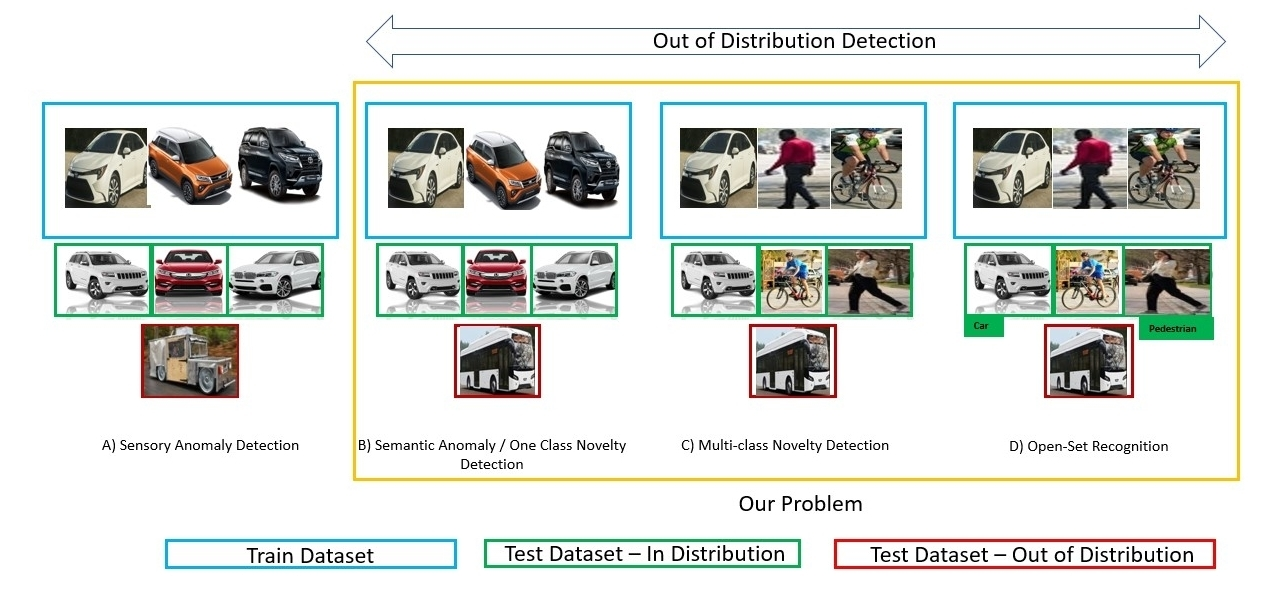
\includegraphics[scale=0.225]{images/OOD_vs_Non-OOD.jpg}
            \caption[\acrlong{ood} detection problem setting]{Class differentiation in generalized OOD detection framework}
            \label{fig:OOD_classes}
        \end{figure}
    \end{itemize}
\end{frame}

\begin{frame}{Out-of-Distribution (OOD) detection(2/3)}
    Different types of OOD data
    \begin{itemize}
        \item Data from a different domain
        \item Data with poor quality of features
        \item Data with inputs that are neither used nor prominent in the training data
    \end{itemize}
\end{frame}

\begin{frame}{Out-of-Distribution (OOD) detection(3/3)}
    Current Object Detection model performance on OOD data
    \begin{figure}[!htbp]
        \centering
      \subcaptionbox{False Positive detection\label{fig:1}}{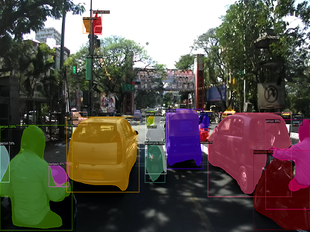
\includegraphics[scale=0.5]{images/False_Positive.png}}%\hspace{1em}
      \subcaptionbox{False Negative detection\label{fig:2}}{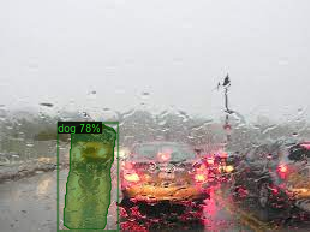
\includegraphics[scale=0.5]{images/False_Negative.png}}
      \caption[Sample False Positive and False Negative detections]{Examples of failures in object dedtection}
      \label{fig:3}
    \end{figure}
\end{frame}

\begin{frame}{OOD detector - Expectations}
    \begin{itemize}
        \item Produce a \textbf{\textit{Novelty Score (NS)}}. 
        \item NS can be a distance metric, a class-dependent probabilistic value, an entropy value, or a descriptive statistic value
        \item OOD detection can be posed as a binary classification problem.

    \end{itemize}
        
    $ X=
        \begin{cases}
            \text{ID}, & \text{if}\ NS \geq \delta \\
            \text{OOD}, & \text{otherwise} 
        \end{cases}
        $
    
% \end{frame}

% \begin{frame}{Novelty Score - Behavior}
    \begin{figure}[H]
        \centering
        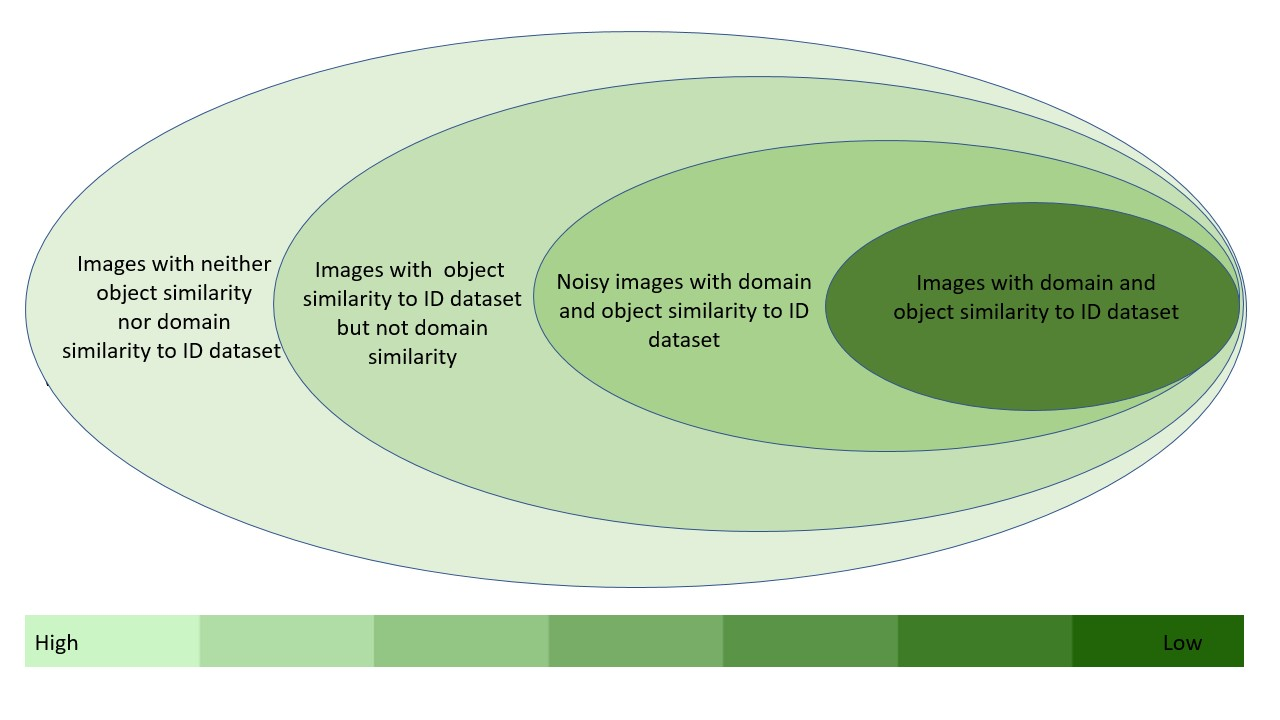
\includegraphics[scale=0.15]{images/Slide2.jpg}
        \caption[Novelty Score behavior]{Expected behavior of novelty score based on the nature of the OOD input}
        \label{fig:OD2_features}
    \end{figure}
\end{frame}

\begin{frame}{Previous works}
    \begin{table}[]
        \centering
        \caption{Previous works on OOD detection}
        \label{tab:my-table}
            \begin{tabular}{ll}
                \textbf{Method}             & \textbf{Works Proposed} \\ \hline
                Metric based methods        & \begin{tabular}[c]{@{}l@{}}\citet{Devries},  \citet{Oberdiek2018}, \\  \citet{Hendrycks2018} , \citet{Lee2018}\end{tabular} \\\hline
                Inconsistency based methods & \citet{liang2017enhancing} \\ \hline
                Generative methods          & \begin{tabular}[c]{@{}l@{}}\citet{Hendrycks2017},  \citet{Ren2019}, \\  \citet{VanDenOord2016}\end{tabular}    \\ \hline
                Uncertainty based methods   & \begin{tabular}[c]{@{}l@{}}\citet{Malinin2018},  \citet{Lakshminarayanan2017}, \\  \citet{VanAmersfoort2020} \\ \end{tabular}                       
            \end{tabular}
    \end{table}
\begin{itemize}
    \item Works only for classification problem
    \item Not directly adaptable to object detection problem   
\end{itemize}
    

    
\end{frame}



\begin{frame}[allowframebreaks]
    \frametitle{References}
    \bibliographystyle{abbrvnat}
    \bibliography{bibliography.bib}
\end{frame}
\end{document}
